\section*{Appendix (Supplementary Material)}
\addcontentsline{toc}{section}{Appendix}
\renewcommand{\thesubsection}{A.\arabic{subsection}}
\renewcommand{\thetable}{A\arabic{table}}\renewcommand{\thefigure}{A\arabic{figure}}
\setcounter{table}{0}\setcounter{figure}{0}
This appendix gives the implementation details needed for reproduction and the complete experimental record behind the
summaries of the main text. All tables and figures are generated by scripts from the raw result files; no number was
entered by hand. The repository additionally contains every metric at every label budget.

\subsection{Benchmark construction}
\label{app:data}
\textbf{Crops.} FUNSD words are cropped from the page with a 2-pixel margin after rescaling
the LayoutLM-normalised boxes ($[0,1000]^2$) of the public Hugging Face release to pixel coordinates;
cropping with the raw values yields misaligned crops for almost every word (the Tesseract word error
rate is 99.8\% without the rescaling and 36.9\% with it). CORD words are cropped from the axis-aligned
bounding box of each word quadrilateral; the official train and validation receipts form the training
pool. SROIE, IAM and IIIT5K are distributed as crops. Crops narrower than 6 or shorter than 8 pixels,
and empty transcriptions, are discarded.

\textbf{Engines.} Tesseract~5.2 (LSTM engine, \texttt{--psm 7}, crops shorter than 32 px are
bicubically upscaled to 32 px) outputs the space-joined words it detects and their mean confidence.
TrOCR-small (\texttt{microsoft/trocr-small-printed} or \texttt{-handwritten}) decodes greedily; its
confidence is the mean token probability.

\textbf{Labels.} A claim is \textsc{Correct} iff it equals the ground truth after whitespace
normalisation (case-insensitive for IIIT5K). No other normalisation is applied, so case and punctuation
errors count as errors, as they do for any downstream consumer that copies the field verbatim.

\textbf{Caveats.} TrOCR's printed checkpoints were fine-tuned on SROIE receipts; the verifier
$V_1$ is therefore in-domain on SROIE, and TrOCR-small makes only 3--6\% errors there, which is why
SROIE uses Tesseract claims. Tesseract is degenerate on handwriting (93.9\% word error on IAM), which is
why IAM uses TrOCR-small claims.


\subsection{Counterfactual neighbourhood generation}
\label{app:graph}
\textbf{Confusion groups.} Substitutions are drawn from the groups
\texttt{O0oQDCc}, \texttt{Il1|!ij}, \texttt{5Ss\$}, \texttt{8B\&3}, \texttt{2Zz}, \texttt{6Gb}, \texttt{9gq},
\texttt{7T/}, \texttt{uvnUV}, \texttt{wW}, \texttt{.,:;'`"}, \texttt{-\_\textasciitilde=}, \texttt{()\{\}[]},
\texttt{aeo}, \texttt{hbk}, \texttt{rnm}, \texttt{cC(e}, \texttt{xX\%}, \texttt{yY}, \texttt{pP}, \texttt{fft}; at most two
alternatives per character are used.

\textbf{Algorithm.} Given claim $h$ and verifier readings $g_1$ (TrOCR) and $g_2$ (PARSeq):
\begin{enumerate}
\item add $g_2$ and $g_1$ (if different from $h$);
\item for each reading, add every single edit of $h$ suggested by its Levenshtein alignment to the
reading: substitution of an aligned mismatching character, deletion of an unaligned character of $h$,
insertion of an unaligned character of the reading;
\item for each position of $h$ (up to 32): a case flip, up to two confusion substitutions, and a deletion;
\item deduplicate, keep insertion order, and stop at $M=28$ neighbours.
\end{enumerate}
No step uses the ground truth. The share of real errors whose truth is a node of the graph is reported
in Table~\ref{tab:truth_in_graph}.

\textbf{Rendering.} $R(v)$ draws $v$ in Liberation Sans (metrically equivalent to Arial) at
$0.75\times$ the crop height (clamped to $[32,96]$ px), black on white, with a quarter-height margin. The
same rendering is fed to both verifiers. PARSeq scores the string restricted to its 94-character
charset and truncated to its maximum label length of 25.


\subsection{Label-free pretraining data}
\label{app:pretrain}
From the unlabeled training pool we keep images on which two independent engines produce the
identical string (Tesseract and TrOCR-small; TrOCR-small and TrOCR-base on IAM), shuffle them with a
fixed seed and keep at most 3{,}000. Each yields a pseudo-correct graph (the agreed string) and, if the
corruption changes the string, a pseudo-incorrect graph built around one or two random OCR-style edits:
confusable substitution (45\%), case flip (15\%), deletion (20\%) or insertion of a confusable character
(20\%). The repair target of a corrupted graph is the node holding the agreed string (when present).
Agreement is a proxy, not ground truth; its precision on the training pool is reported in
Table~\ref{tab:pretrain_stats}.

\begin{table}[htbp]\centering
\caption{Label-free pretraining sets. Precision of engine agreement is measured post hoc against the
ground truth of the training pool (never used for training).}
\label{tab:pretrain_stats}
\scriptsize\begin{tabular}{lcccc}\toprule
Dataset & agreeing images & graphs & precision of agreement & truth in graph (corruptions) \\\midrule
\tabinput{tables/pretrain_stats.tex}
\bottomrule\end{tabular}\end{table}


\subsection{Hyperparameters and baseline protocols}
\label{app:hparams}
\begin{table}[htbp]\centering\caption{Hyperparameters (identical for all datasets and all $k$).}
\scriptsize\resizebox{\linewidth}{!}{\begin{tabular}{ll}\toprule
Node features & $2\times11$ evidence + 7 claim deltas ($\tanh$-squashed) + 8 edit-kind + 1 position + 6 agreement (claim node)\\
Edge features & 8 edit kinds + sibling + path + self (one-hot)\\
GNN & 3 GATv2 layers, hidden 64, 4 heads, residual + LayerNorm, dropout 0.2\\
Readout & claim state, attention pool, max pool over rivals, $\beta\log P_{\mathrm{opt}}$ ($\beta$ learned)\\
Pretraining & 15 epochs, AdamW lr $10^{-3}$, wd $10^{-4}$, batch 64, $\lambda=0.5$\\
Few-shot fine-tuning & 300 steps, AdamW lr $3\cdot10^{-4}$, batch $\min(64,k)$, class-balanced BCE\\
Head selection & repeated stratified CV (3 repeats, $\le$5 folds) on the support only; fusion if $\min$ class $<5$\\
Anchored head & priors scaled $\times10$; residual $\ell_2$ LR, $C\in\{.003,.01,.03,.1,.3\}$ by CV on the support\\
Full supervision & 60 epochs, early stopping (patience 8) on a 15\% split of the training pool\\
Seeds & 0--4 (support sampling, initialisation, pretraining)\\
\bottomrule\end{tabular}}\end{table}

\textbf{Thresholds.} Engine confidence and the $\rho$-margin rule are thresholded at the value
maximising macro-F1 on the $k$-shot support (seed-specific). Agreement baselines are binary
(accept iff equal). The graded PARSeq score is $+c$ if PARSeq's reading equals the claim and $-c$
otherwise, where $c$ is PARSeq's sequence confidence (product of character probabilities); it is
thresholded at 0, which coincides with the binary decision.

\textbf{VLM judge prompt.} \emph{Does the image show exactly the text "\{claim\}" (same characters,
case and punctuation)? Answer yes or no.} The image is passed at its native resolution (upscaled to a
height of 56 px if smaller; Qwen2.5-VL pixel budget 32--256 visual tokens). The score is the
renormalised probability of \texttt{yes}/\texttt{Yes} versus \texttt{no}/\texttt{No} as the first
generated token.

\textbf{ConfidNet-style learned confidence.} A one-hidden-layer MLP (32 units, $\ell_2$ $10^{-2}$)
on the engine confidence and five likelihood statistics of the claim under TrOCR-base, trained on the
support set.


\subsection{Additional analyses and qualitative examples}
\label{app:extra}
\subsection*{Error types}
Table~\ref{tab:error_types} breaks down the detection rate (recall of truly incorrect claims) by the edit that
separates the claim from the truth. Operating points: \ours{} at $P=0.5$, PARSeq-graded at its natural
threshold, the VLM at 0.5, and engine confidence at its \emph{test-optimal} threshold (favourable to the baseline).
\begin{table}[htbp]\centering
\caption{Detection rate (\%) by error type; number of errors of that type in parentheses ($k=25$).}
\label{tab:error_types}
\scriptsize\setlength{\tabcolsep}{3pt}\begin{tabular}{llccccc}\toprule
Dataset & Method & substitution & insertion & deletion & case only & multi-edit\\\midrule
\tabinput{tables/error_types.tex}
\bottomrule\end{tabular}\end{table}

\subsection*{Claim length}
\begin{figure}[htbp]\centering
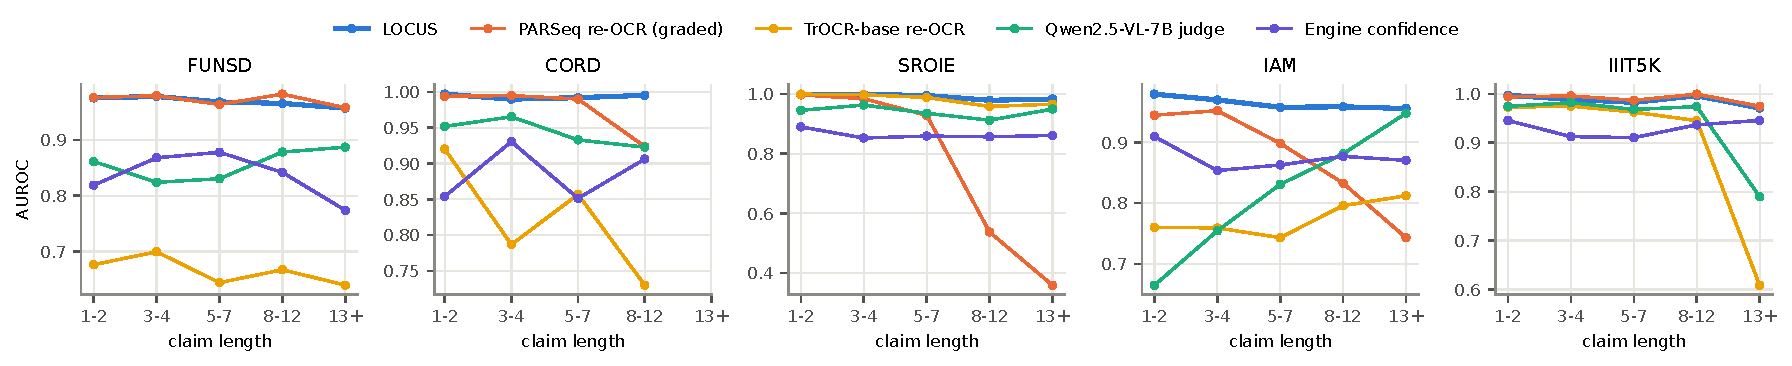
\includegraphics[width=\linewidth]{figs/by_length.pdf}
\caption{AUROC by claim length ($k=25$). Bins with fewer than 30 words or a single class are omitted.}
\label{fig:by_length}
\end{figure}

\subsection*{Calibration}
\begin{table}[htbp]\centering
\caption{Expected calibration error (15 bins) of the correctness probability ($k=25$; PARSeq-graded mapped
to $[0,1]$ as $(s+1)/2$). Lower is better.}
\label{tab:calibration}
\scriptsize\begin{tabular}{lcccc}\toprule
Dataset & \ours{} & PARSeq graded & Qwen2.5-VL-7B & Engine conf.\\\midrule
\tabinput{tables/calibration.tex}
\bottomrule\end{tabular}\end{table}

\subsection*{AUROC and AURC learning curves}
\begin{figure}[htbp]\centering
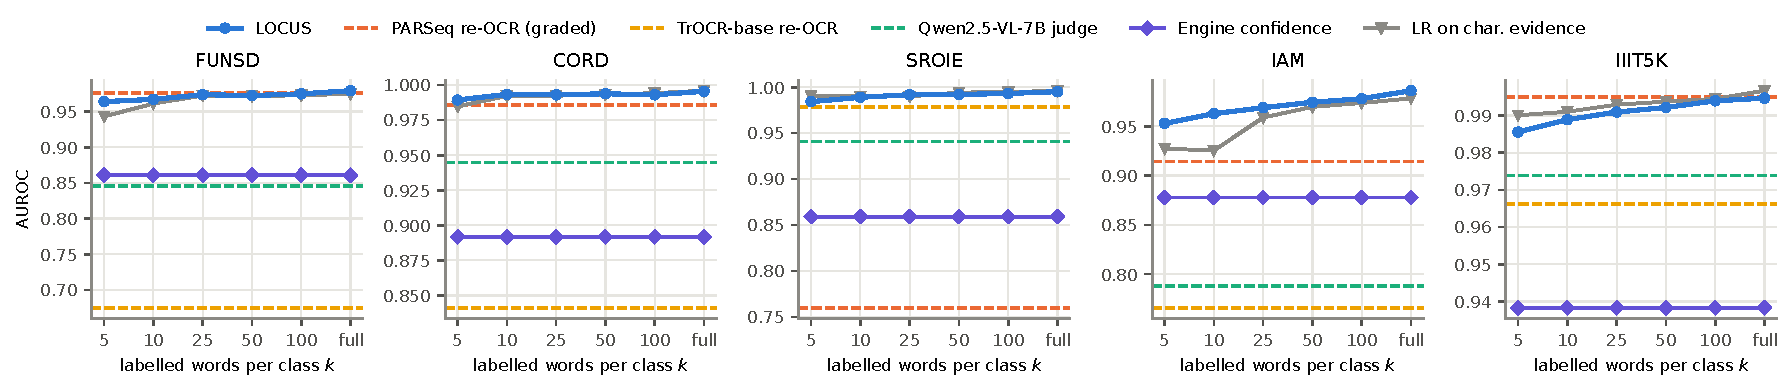
\includegraphics[width=\linewidth]{figs/learning_curves_auroc.pdf}
\caption{AUROC as a function of the number of labelled words per class (ensembles of five seeds;
dashed: label-free baselines).}
\label{fig:lc_auroc}
\end{figure}

\subsection*{Cross-dataset transfer (AUROC)}
\begin{table}[htbp]\centering
\caption{Cross-dataset transfer, AUROC (rows: training dataset, fully supervised; columns: test dataset;
diagonal: in-domain).}
\label{tab:xds_auroc}
\scriptsize\begin{tabular}{lccccc}\toprule
Train $\backslash$ Test & FUNSD & CORD & SROIE & IAM & IIIT5K\\\midrule
\tabinput{tables/xdataset_auroc.tex}
\bottomrule\end{tabular}\end{table}

\subsection*{Ablations: AUROC and repair}
\begin{table}[htbp]\centering
\caption{Ablations at $k=25$, AUROC (ensemble of five seeds). Last column: mean change w.r.t.\ the full model.}
\label{tab:ablation_auroc}
\scriptsize\begin{tabular}{lcccccc}\toprule
Variant & FUNSD & CORD & SROIE & IAM & IIIT5K & $\Delta$\\\midrule
\tabinput{tables/ablation_auroc.tex}
\bottomrule\end{tabular}\end{table}

\subsection*{Sensitivity}
\begin{table}[htbp]\centering
\caption{Sensitivity of \ours{} ($k=25$, ensemble of five seeds) to the size of the label-free pretraining
set, the number of fine-tuning steps, and the support-selection strategy (label-free $k$-means clusters the
unlabeled pool in the pretrained embedding space and labels the $2k$ medoids).}
\label{tab:sensitivity}
\scriptsize\begin{tabular}{llcccccc}\toprule
& & \multicolumn{2}{c}{FUNSD} & \multicolumn{2}{c}{CORD} & \multicolumn{2}{c}{IAM}\\
Factor & Value & F1 & AUROC & F1 & AUROC & F1 & AUROC\\\midrule
\tabinput{tables/sensitivity.tex}
\bottomrule\end{tabular}\end{table}

\subsection*{Main comparison at other label budgets and metrics}
\newcommand{\maintab}[3]{\begin{table}[p]\centering\caption{#2}\label{#3}
\scriptsize\setlength{\tabcolsep}{4pt}\resizebox{\linewidth}{!}{\begin{tabular}{lcccccc}\toprule
Method & FUNSD & CORD & SROIE & IAM & IIIT5K & Avg.\\\midrule
\tabinput{tables/#1.tex}
\bottomrule\end{tabular}}\end{table}}
\maintab{main_macro_f1_k10}{Macro-F1 at $k=10$ (protocol of Table~\ref{tab:main}).}{tab:main_f1_k10}
\maintab{main_macro_f1_k100}{Macro-F1 at $k=100$.}{tab:main_f1_k100}
\maintab{main_macro_f1_kfull}{Macro-F1 with full supervision (85\% of the training pool; 15\% for early stopping).}{tab:main_f1_full}
\maintab{main_auroc_k10}{AUROC at $k=10$.}{tab:main_auc_k10}
\maintab{main_auroc_k100}{AUROC at $k=100$.}{tab:main_auc_k100}
\maintab{main_aurc_k25}{AURC at $k=25$ (lower is better; best = lowest).}{tab:main_aurc_k25}
\maintab{main_cov@95_k25}{Coverage at 95\% accepted precision at $k=25$ (higher is better).}{tab:main_cov_k25}

\subsection*{Composition of real OCR errors}
\begin{figure}[htbp]\centering
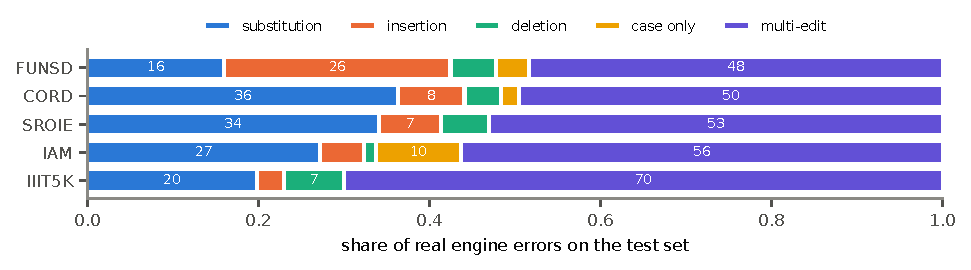
\includegraphics[width=0.85\linewidth]{figs/error_type_dist.pdf}
\caption{Types of real engine errors on each test set (share of errors; labels for shares above 7\%).
Handwriting and receipt lines are dominated by multi-edit errors, which bounds what a single-edit
neighbourhood can repair (Table~\ref{tab:truth_in_graph}).}
\label{fig:error_type_dist}
\end{figure}

\begin{figure}[htbp]\centering
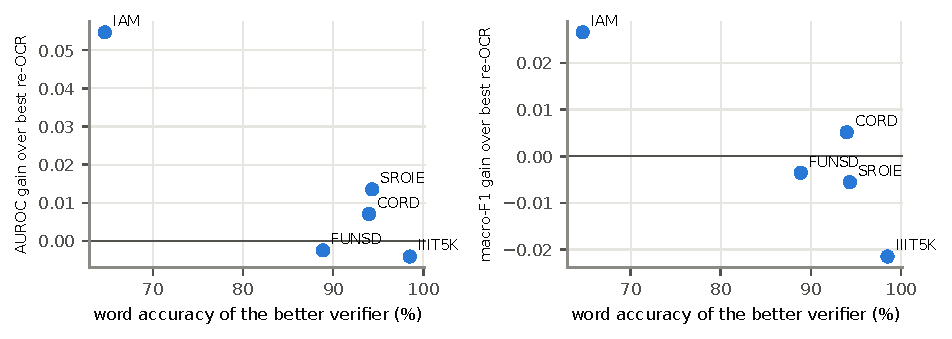
\includegraphics[width=0.75\linewidth]{figs/recog_dependence.pdf}
\caption{Gain of \ours{} over the best re-recognition baseline against the word accuracy of the better verifier (one
point per dataset).}
\label{fig:recog}
\end{figure}
\begin{figure}[htbp]\centering
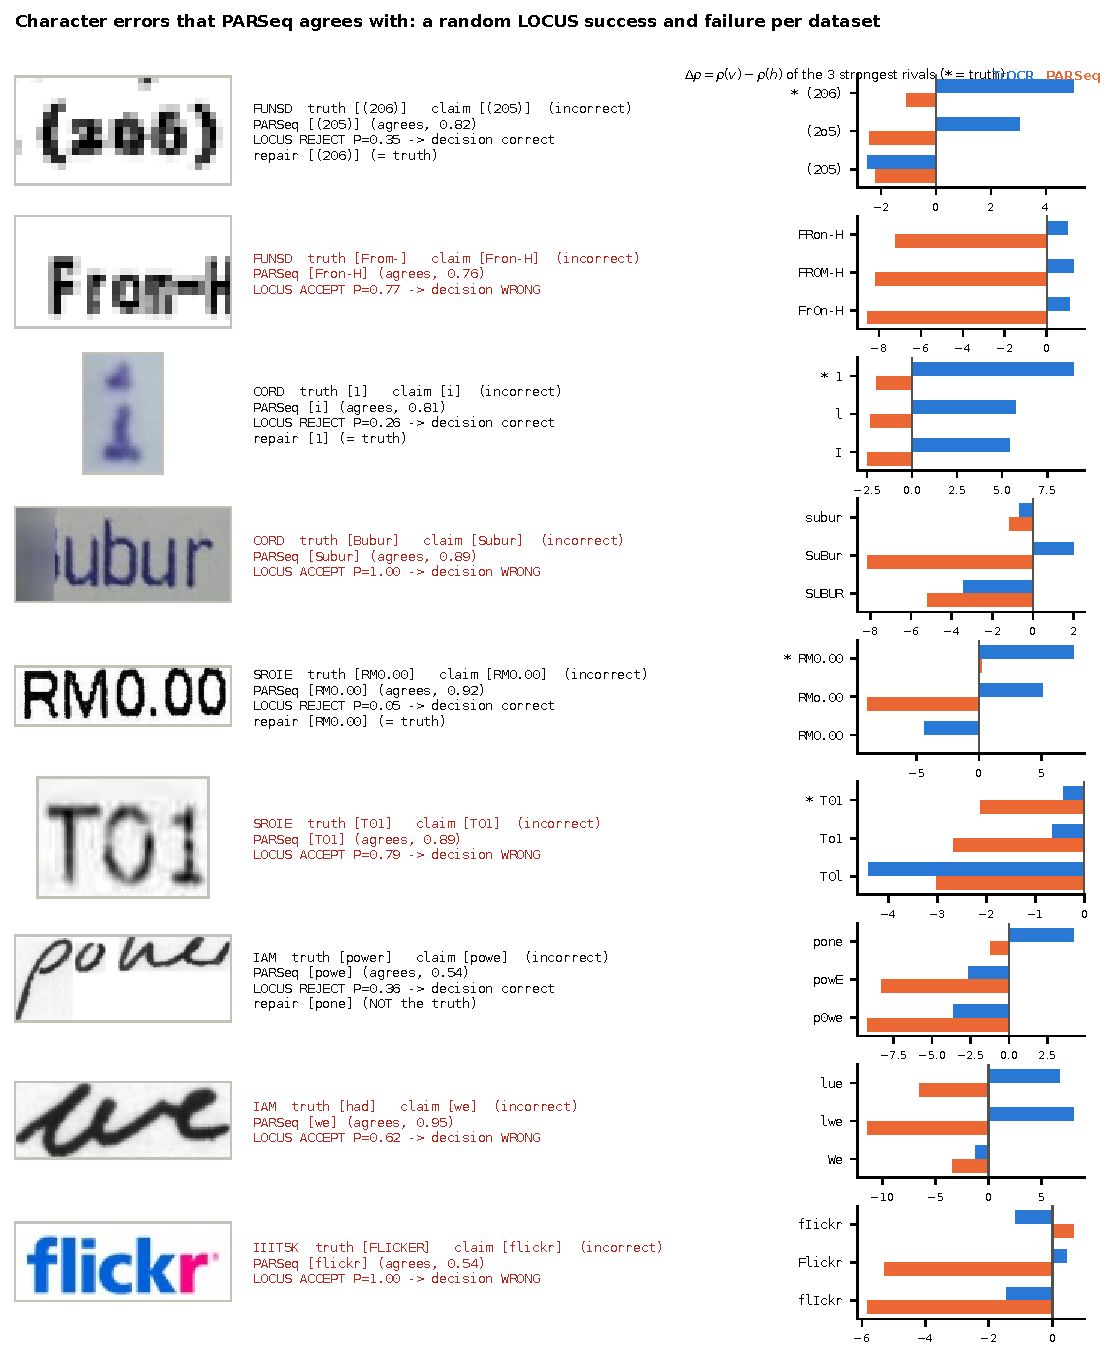
\includegraphics[width=0.8\linewidth]{figs/qual_regime_fooled.pdf}
\caption{\textbf{Errors that PARSeq re-recognition accepts} (it reads the same string as the engine), restricted to
genuine character errors (case-only and punctuation-only differences excluded): for each dataset one random
\ours{} success and one random failure. \ours{} rejects only a small fraction of this stratum
(Table~\ref{tab:qual_counts}); the manual audit (Table~\ref{tab:audit}) shows why: most of these ``errors'' are
annotation or cropping problems, i.e.\ the claim matches what is visible.}
\label{fig:qual_fooled}
\end{figure}

\begin{figure}[htbp]\centering
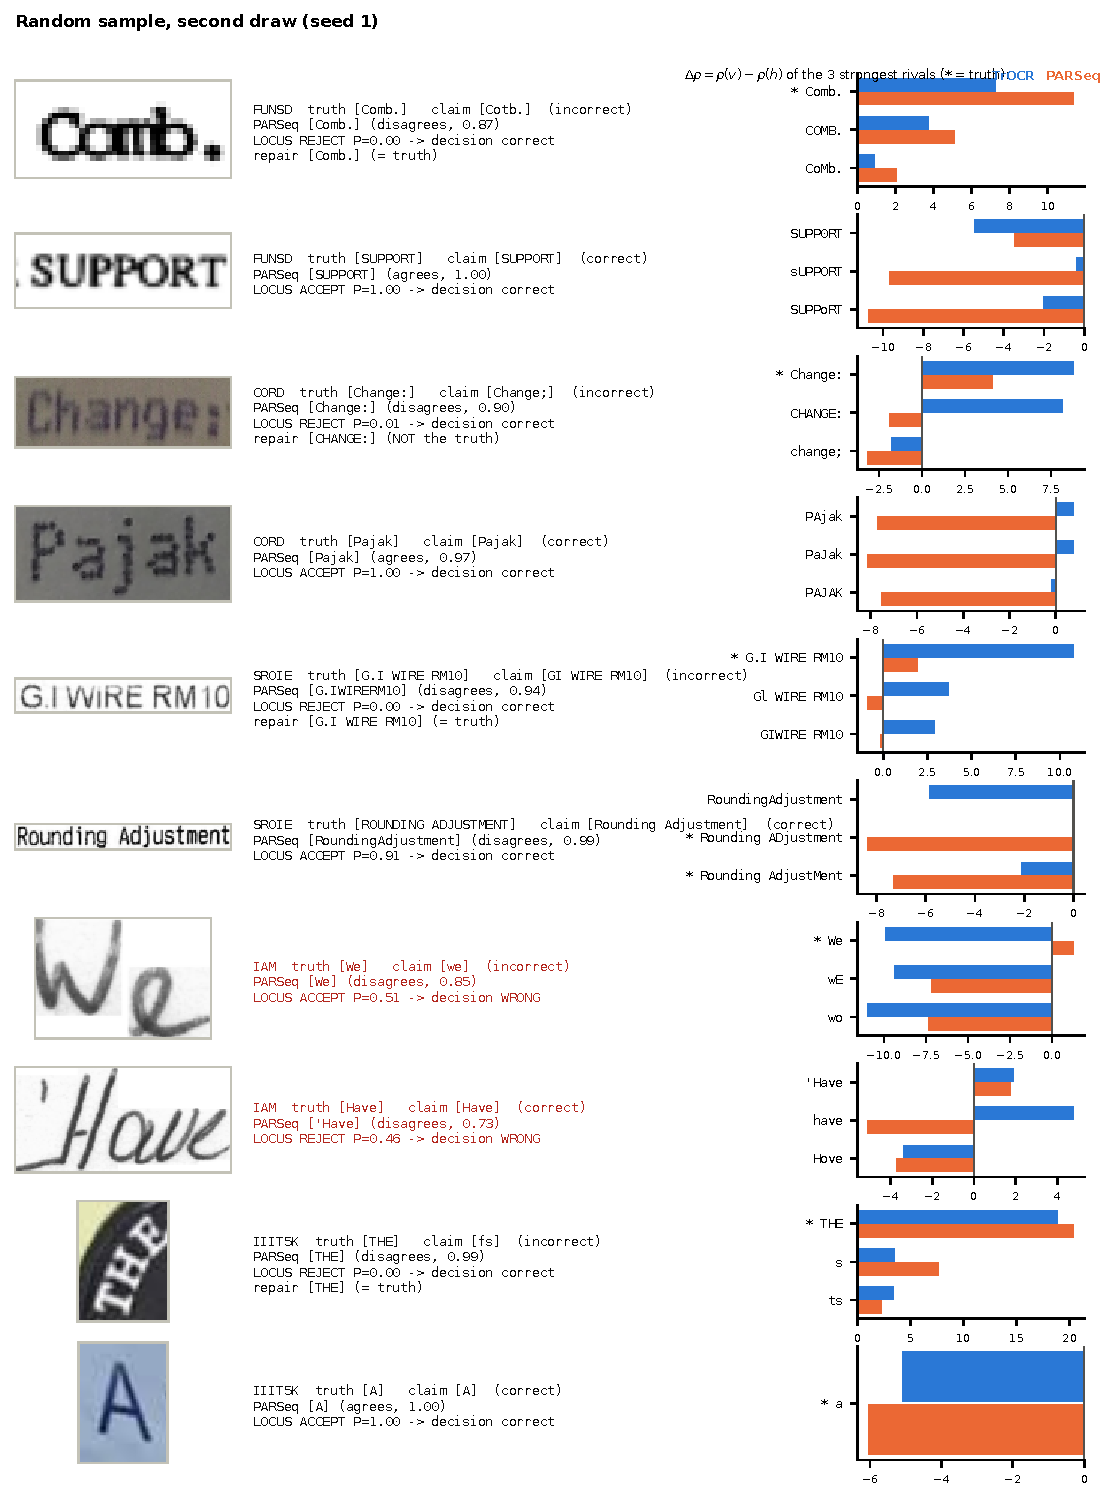
\includegraphics[width=0.8\linewidth]{figs/qual_random2.pdf}
\caption{\textbf{Second random sample} (seed 1), same protocol as Fig.~\ref{fig:qual_random}.}
\label{fig:qual_random2}
\end{figure}

\begin{figure}[htbp]\centering
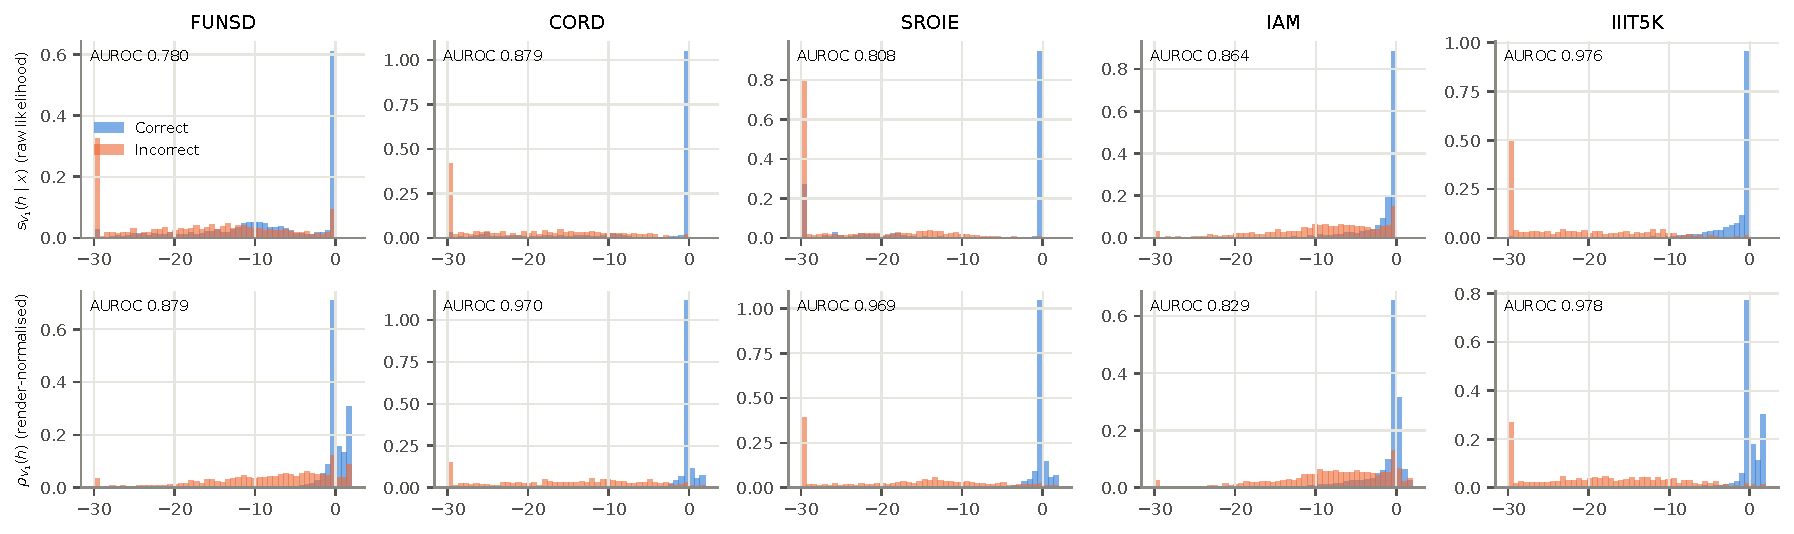
\includegraphics[width=0.92\linewidth]{figs/rho_separation.pdf}
\caption{\textbf{Render normalisation on real data.} Distribution of the claim's raw TrOCR likelihood (top) and of its
render-normalised ratio $\rho$ (bottom) for correct and incorrect claims, with the AUROC of each single score.}
\label{fig:rho}
\end{figure}

\begin{table}[htbp]\centering
\caption{\textbf{Single-verifier setting} (no agreement features), $k=25$, macro-F1: effect of render normalisation
when only one recogniser is available.}
\label{tab:single}
\footnotesize\begin{tabular}{lccccc}\toprule
Variant & FUNSD & CORD & SROIE & IAM & IIIT5K\\\midrule
\tabinput{tables/ablation_single.tex}
\bottomrule\end{tabular}\end{table}

\subsection{Full results}
\label{app:full}
Tables~\ref{tab:k_macro_f1_FUNSD}--\ref{tab:all_IIIT5K_k25} report every method at every $k$ with seed standard
deviations, and every metric at $k=25$.

\tabinput{tables/kgrid_macro_f1.tex}
\tabinput{tables/kgrid_auroc.tex}
\tabinput{tables/all_metrics_k25.tex}
